\documentclass[10pt]{article}
\usepackage[letterpaper,margin=0.82in]{geometry}
\usepackage[T1]{fontenc}
\usepackage{lmodern,microtype}
\usepackage{amsmath,amssymb,mathtools,booktabs,graphicx}
\usepackage[numbers,sort&compress]{natbib}
\usepackage{xcolor,caption,xspace}
\usepackage[colorlinks=true,allcolors=blue!45!black]{hyperref}
\captionsetup{font=small,labelfont=bf}
\setlength{\parskip}{2pt}\setlength{\parindent}{1em}
\setlength{\emergencystretch}{2em}
\clubpenalty=10000\widowpenalty=10000
\newcommand{\FNorm}[1]{\left\lVert #1\right\rVert_F}
\newcommand{\SN}[1]{\left\lVert #1\right\rVert_2}
\newcommand{\R}{\mathbb{R}}
\newcommand{\SAND}{\textsc{Sand-Muon}\xspace}

\title{\SAND: Inexpensive Sensitivity Geometry for Spectral Optimization}
\author{Hamza Kharbouch\\Independent Researcher, Morocco\\\texttt{hamza.kharbouch.work@gmail.com}}
\date{Preliminary research manuscript}

\begin{document}
\maketitle

\begin{abstract}
Muon applies a spectral transformation to matrix momentum, but its isotropic polar target ignores the different scales of layer inputs and output sensitivities. We study \SAND, a practical two-sided geometry for Muon built from diagonal activation second moments and diagonal squared real-loss cotangents, with the activation side retaining one exact rank-one mean correction. For each layer, the resulting small-statistic preconditioners whiten the momentum before a compensated five-stage S8 map and are paired with a transpose-aware map-back. The rank-one correction admits analytic vector actions, avoiding dense covariance factors. In one 103.2M-parameter GPT-2-style FineWeb-Edu run on an RTX 3090, \SAND reaches validation loss 3.277938 after 15,106 updates and 1.980B tokens in 37,808.94 recorded training seconds. An archived Polar Express run records loss 3.304063 after 16,000 updates and 2.097B tokens in 37,807.67 seconds. This is a descriptive comparison at nearly equal recorded training durations. Token counts differ, the runs do not form a same-host speed study, and the recipes differ in momentum, polarization, auxiliary optimizer, and schedule; each method has one seed. A separate centered-FP32 pilot screens several geometries but does not validate the production BF16 recipe. These observations motivate controlled follow-up work; they do not establish that the proposed statistics caused the loss difference or that \SAND is generally superior.
\end{abstract}

\section{Introduction}
Muon orthogonalizes a matrix momentum buffer before using it to update a hidden-layer matrix \citep{jordan2024muon,liu2025scalable}. In exact arithmetic, if $G=U\Sigma V^\top$, the polar factor $Q=UV^\top$ solves
\begin{equation}\label{eq:polar-oracle}
 Q\in\arg\max_{\SN{D}\leq 1}\langle G,D\rangle,
 \qquad \langle G,Q\rangle=\|G\|_* .
\end{equation}
This is a precise first-order statement under a spectral-norm constraint. It does not say that all layer directions have equal curvature, that the exact polar update is optimal over a training trajectory, or that a finite polynomial implementation attains the oracle.

\SAND asks whether inexpensive per-layer signals can supply a useful coordinate system before this spectral step. For a linear map with input activation $x$ and output cotangent $\delta$, the method maintains (i) input-channel second moments and means, and (ii) output-channel squared cotangents from the observed loss. The input statistic is represented as a diagonal centered variance plus a rank-one mean outer product. Its nonsymmetric whitening factor has an analytic diagonal-plus-vector action, and the transpose is used in map-back. The output statistic is diagonal. Both factors are updated from the full effective batch with a fixed exponential moving average (EMA) coefficient of $0.97$.

The production recipe combines these estimates with $0.8$ Nesterov matrix momentum, a compensated BF16 five-stage S8 polarizer, and a final Frobenius graft that restores the matrix-step scale. The geometry is layerwise and data dependent, while the polynomial recipe remains shared. This study is a system-and-method report: it documents the exact production recipe, relates its idealized weighted polar map to existing curvature-aware Muon methods, and reports a single FineWeb-Edu run alongside a small screening pilot. It does not isolate the contributions of the activation correction, cotangent weighting, momentum, or finite-precision polarizer.

\paragraph{Contributions.} (1) We give an analytic rank-one representation of a non-centered activation second-moment geometry and describe its use around a finite spectral update. (2) We state the corresponding exact weighted spectral oracle and distinguish it from the deployed approximate, momentum-based update. (3) We document a 103M-parameter FineWeb-Edu case study at nearly equal recorded training durations and a small centered-FP32 screening panel, with comparison limits stated alongside the results.

\section{Relation to prior work}
Muon's polar update follows a steepest-descent interpretation under a spectral constraint, while practical implementations approximate the polar map with Newton--Schulz polynomials \citep{jordan2024muon,liu2025scalable}. Polar Express (PE) improves finite-stage polynomial behavior through coefficient construction and stable normalization \citep{amsel2025polar}. S8 uses a separate five-stage fit with compensated first-stage BF16 products; it is part of the deployed recipe here, not the methodological novelty claimed for \SAND. The normalization draws on prior work, while the fitted S8 recipe and implementation are documented in the S8Muon research artifact \citep{s8muon,grishina2025cans}.

Curvature-aware spectral optimizers provide the closest context. K-FAC and Shampoo use structured matrix statistics to precondition gradients or momentum \citep{martens2015kfac,gupta2018shampoo}; SOAP combines Shampoo-like preconditioning with an orthogonalized basis \citep{vyas2024soap}. FISMO formulates a Fisher-structured momentum-orthogonalized update, and Mousse applies a polar map in Shampoo-induced whitened coordinates \citep{xu2026fismo,zhang2026mousse}. GO-Muon gives a weighted spectral oracle for general positive-definite left and right maps \citep{che2026gomuon}. These works establish important conceptual overlap: anisotropic geometry can be paired with spectral optimization, and a whitened polar oracle is not unique to this manuscript.

The most direct diagonal comparison is MALT, which uses two-sided diagonal preconditioning, a Newton--Schulz transform, and norm grafting \citep{wu2026malt}. Its published construction is not identical to ours. MALT accumulates row- and column-wise squared norms of the aggregate gradient matrix and uses an inverse eighth-power preconditioner. SAND instead estimates the input factor from activations and the output factor from per-channel squared real-loss cotangents, with inverse-square-root scaling and a rank-one input mean term. The EMA coefficient is $0.97$, matrix momentum is $0.8$, and polarization uses the compensated S8 recipe. MALT reports a different statistic EMA ($0.99$) and matrix momentum ($0.95$) in the referenced version. Thus SAND is a distinct implementation and statistical choice within the same broad two-sided preconditioning family, not a claim to originate weighted polar optimization.

For a linear layer, the aggregate gradient is proportional to $N^{-1}\sum_n\delta_n x_n^\top$. Cancellation between examples can alter its row and column energies while leaving the separate squared activation and cotangent moments unchanged. The methods therefore use different information, not just different powers of one statistic. This distinction motivates a direct comparison; it does not itself prove that either geometry is a better curvature approximation.

The activation and cotangent summaries have a curvature motivation. Their factorized product is not, in general, the exact empirical Fisher or the model Fisher. Second moments of layer inputs and output derivatives resemble the two factors used in Kronecker-factored curvature methods. Here they supply coordinate scales for a spectral map; we do not establish equality to a Hessian or generalized Gauss--Newton matrix. In particular, the output statistic uses the cotangent produced by the observed labels, not a model-sampled or all-label expectation. FineWeb-Edu supplies the language-model training data for the case study \citep{penedo2024fineweb}.

\section{Method}
\subsection{Layerwise statistics}
Consider a hidden linear map $y=W x$, with $W\in\R^{o\times d}$, input rows $x_n\in\R^d$, and output cotangents $\delta_n\in\R^o$ over the effective batch. For each input channel $j$, define batch moments
\begin{equation}
 m_j=\frac1N\sum_{n=1}^N x_{n,j},\qquad
 s_j=\frac1N\sum_{n=1}^N x_{n,j}^2.
\end{equation}
The activation geometry is
\begin{equation}\label{eq:A}
\begin{aligned}
 q&=\max\left(\operatorname{mean}(s^{\rm EMA}),\mathrm{tiny}\right),
 &\widetilde m&=m^{\rm EMA}/\sqrt q,\\
 d_j&=\max\left(\frac{s_j^{\rm EMA}-(m_j^{\rm EMA})^2}{q},10^{-6}\right),
 &A&=\operatorname{diag}(d)+\widetilde m\widetilde m^\top.
\end{aligned}
\end{equation}
It includes the mean outer product while retaining only the diagonal of the centered covariance. The scalar $q$ normalizes the EMA raw second moments, and $\mathrm{tiny}$ denotes the smallest normal FP32 value used by the implementation. Therefore $A$ is generally different from both the diagonal of the raw second moment and the full activation covariance.

For output channels, let $r_i=N^{-1}\sum_n\delta_{n,i}^2$. We normalize each nonzero batch vector by its channel mean, $\bar r_i=r_i/\operatorname{mean}(r)$, and maintain its EMA $r^{\rm EMA}$. The output factor is
\begin{equation}
 B=\operatorname{diag}(b),\qquad
 b_i=\max\left(\frac{r_i^{\rm EMA}}{\operatorname{mean}(r^{\rm EMA})},10^{-6}\right).
\end{equation}
The activation second-moment and mean vectors use the same EMA coefficient. In both cases the first batch initializes the state; subsequent updates use
\begin{equation}\label{eq:ema}
 z_t=\beta z_{t-1}+(1-\beta)\widehat z_t,\qquad \beta=0.97.
\end{equation}
Statistics are accumulated over all microbatches in one optimizer update. The attention query, key, and value projections share the same input geometry because they consume the same activation. The real-loss cotangent statistic is tracked separately for each output projection.

For numerical stability, the implementation scales channel variances by the mean raw second moment and floors normalized diagonal entries at $10^{-6}$ before inverse-square-root operations. The cotangent geometry is normalized to mean one before applying the same relative floor. These conventions make the preconditioners dimensionless while bounding diagonal amplification. They are implementation safeguards, not claims that the underlying empirical covariance is nonsingular.

\subsection{Analytic rank-one whitening}
Let $D=\operatorname{diag}(d)$ and define $z=D^{-1/2}\widetilde m$. Then
\begin{equation}
 A=D^{1/2}(I+zz^\top)D^{1/2}.
\end{equation}
The rank-one matrix $I+zz^\top$ has one exceptional eigenvalue $1+\|z\|^2$ and eigenvalue one on the orthogonal complement. Its inverse square root is
\begin{equation}\label{eq:rank1}
 (I+zz^\top)^{-1/2}=I-\kappa zz^\top,\quad
 \kappa=\frac{1}{\sqrt{1+\|z\|^2}\left(1+\sqrt{1+\|z\|^2}\right)}.
\end{equation}
Define $C=I-\kappa zz^\top$ and the nonsymmetric whitening factor $L_A=CD^{-1/2}$. Although $L_A$ is generally not symmetric, it satisfies $L_A^\top L_A=A^{-1}$. The implementation applies $L_A$ on one side and its transpose on the other where required; it evaluates both actions as diagonal scaling plus vector inner products, without materializing an $O(d^2)$ matrix. This factorization is exact for the represented rank-one model up to the stated floors and floating-point arithmetic; it is not an approximation to the full covariance beyond that model.

Let $L_A$ be the nonsymmetric input whitening factor and $L_B=B^{-1/2}$ the diagonal output factor. For matrix momentum source $M_t$, SAND forms
\begin{equation}\label{eq:white}
 \widetilde M_t=L_B M_t L_A^\top,\qquad
 Q_t^{(8)}=\mathcal{S}_8(\widetilde M_t),\qquad
 U_t=L_B^\top Q_t^{(8)}L_A,
\end{equation}
Here $L_B=B^{-1/2}$ is diagonal and symmetric, while $L_A$ is the nonsymmetric factor above. The transpose in the map-back is consequential: it pairs the transformed matrix with its whitening map. The implementation orients matrices to keep the polynomial's Gram matrix on the smaller dimension, then maps the result back to the stored weight orientation. It applies the validated compensated five-stage S8 transform in whitened coordinates and forms the final matrix direction as $\Delta_t=\sqrt{o}\,U_t/\FNorm{U_t}$. The weight update is $W_{t+1}=W_t-\eta_t\Delta_t$. This Frobenius graft fixes the matrix-step scale; it does not make the finite map an exact polar factor or preserve an arbitrary anisotropic trust-region radius.

\subsection{Exact weighted oracle and scope of the argument}
For fixed nonsingular whitening factors $L_A$ and $L_B$ satisfying $L_A^\top L_A=A^{-1}$ and $L_B^\top L_B=B^{-1}$, define the spectral constraint
\begin{equation}
 \SN{L_B^{-\top} U L_A^{-1}}\leq 1.
\end{equation}
With $Z=L_B G L_A^\top$ and $X=L_B^{-\top}UL_A^{-1}$, the Frobenius pairing obeys $\langle G,U\rangle=\langle Z,X\rangle$. Hence the exact maximizer is
\begin{equation}\label{eq:weighted}
 U_\star=L_B^\top\operatorname{Polar}(Z)L_A,\qquad
 \max_{\SN{L_B^{-\top}UL_A^{-1}}\leq1}\langle G,U\rangle=\|Z\|_*.
\end{equation}
This follows directly from the ordinary polar oracle in Equation~\eqref{eq:polar-oracle}. It is a change-of-variables identity, not a new theorem.

The production method substitutes a momentum source for the current gradient, estimates $A$ and $B$ from a finite batch, refreshes these estimates every update, uses finite-stage S8 in BF16 with compensated products, and then applies a Frobenius graft. Therefore Equation~\eqref{eq:weighted} characterizes the idealized map that motivates the coordinates. It does not establish alignment of the deployed update with the current gradient: momentum can point elsewhere, the finite S8 output is not exactly polar, and the post-map graft and learned dynamics affect the actual step. No convergence guarantee or coordinate invariance is claimed.

\subsection{Momentum and auxiliary parameters}
For each matrix weight, the implementation maintains the exponential momentum $P_t=0.8P_{t-1}+0.2g_t$ and uses the Nesterov source $M_t=0.8P_t+0.2g_t$. The matrix learning rate peaks at $0.01$ and uses a warmup occupying the fraction $100/16{,}000$ of the recorded duration, then follows the time-budget cosine schedule described in Section~\ref{sec:experiment}. PE instead warms up for 100 optimizer updates. Non-matrix parameters use AdamW \citep{loshchilov2017adamw} with learning-rate ratio $0.1$, $\beta_1=0.9$, $\beta_2=0.999$, and weight decay $0.01$.

\section{Experimental case study}\label{sec:experiment}
\subsection{Production run and comparison record}
The production run trains a 103,176,192-parameter decoder-only GPT-2-style model: nine layers, width 768, twelve attention heads, context 1,024, vocabulary 50,257, learned absolute positional embeddings, tied token embedding and output head, pre-LayerNorm, biases, GELU MLP width 3,072, and no dropout. It uses seed 1337, a global batch of 128 sequences in microbatches of 16, and the pinned FineWeb-Edu GPT-2-token shard revision \texttt{a33f75d78c7f74236fb03754ec1eb3cc77507d64}. Each update processes 131,072 target tokens. The SAND run uses one NVIDIA RTX 3090, PyTorch 2.6.0+cu124, FP32 parameters and optimizer states, BF16 autocast forward/backward and BF16 S8 products. SAND's first S8 stage uses compensated products with FP32 accumulators and temporaries.

The candidate was assigned the archived PE run's recorded training-duration budget. Its learning rate follows a cosine in accumulated optimizer-update time, with warmup occupying $100/16{,}000$ of the budget (about 236 s on this run, or about 94 updates). Validation was checked every 2,000 updates against PE loss linearly interpolated at the same recorded training duration; a worse check would stop the run immediately. The seven checks from 2,000 through 14,000 updates all remained below the reference, and the run ended at the time budget. The archived PE reference uses a 16,000-update cosine schedule. Both run manifests report the same model size, seed, dataset revision, context, batch, peak matrix learning rate, validation set protocol, GPU model, and PyTorch version. The comparison still changes several substantive fields: SAND uses $0.8$ matrix momentum, S8 polarization and the geometry described above, AdamW ratio $0.1$ with $\beta_2=0.999$ and decay $0.01$, and a wall-clock schedule. PE uses $0.95$ momentum, its published five-stage polynomial, no geometry weighting, and AdamW ratio $0.1$ with $\beta_2=0.95$ and zero decay. The runs are independent and have no paired random seeds beyond the same initialization seed value.

The recorded time counts synchronized training updates and data transfer, but excludes evaluation, checkpoint I/O, startup, and discarded compilation warmup. The SAND campaign stops at 15,106 updates, 1,979,973,632 tokens, and 37,808.9417 s. The PE archive records 16,000 updates, 2,097,152,000 tokens, and 37,807.6723 s. Thus the recorded update times differ by 1.27 s, while token counts differ by 117,178,368. We treat endpoint validation loss as a descriptive comparison at nearly equal recorded durations. Token counts differ, and this is not a controlled same-host time-to-loss benchmark.

\subsection{Endpoint observations}
\begin{table}[t]
\centering
\caption{Available single-run endpoint observations. Validation loss is mean next-token negative log-likelihood in nats; S8Muon and vanilla Muon are included only as historical context from the S8 paper and do not isolate SAND's geometry.}
\label{tab:endpoints}
\begin{tabular}{lrrr}
\toprule
Method & Updates & Tokens (B) & Final loss\\
\midrule
PE (archived reference) & 16,000 & 2.097 & 3.304063\\
Vanilla Muon (historical context) & 16,000 & 2.097 & 3.310583\\
S8Muon (historical context) & 16,000 & 2.097 & 3.301541\\
\SAND (production run) & 15,106 & 1.980 & 3.277938\\
\bottomrule
\end{tabular}
\end{table}

At nearly equal recorded training durations, SAND's endpoint validation loss is $0.026125$ nats below the archived PE value. The SAND campaign's terminal loss is also its lowest recorded validation loss. The difference is descriptive and belongs to the complete recipes. The archived S8Muon and vanilla-Muon outcomes contextualize the earlier 103M experiment; they differ from the present run in optimizer recipe and schedule and do not isolate geometry. No uncertainty interval is available from independent seeds. The fixed validation prefix is repeatedly evaluated and also serves as a stopping guard, so it is a monitored validation series rather than a blind test set.

\begin{figure}[!htbp]\centering
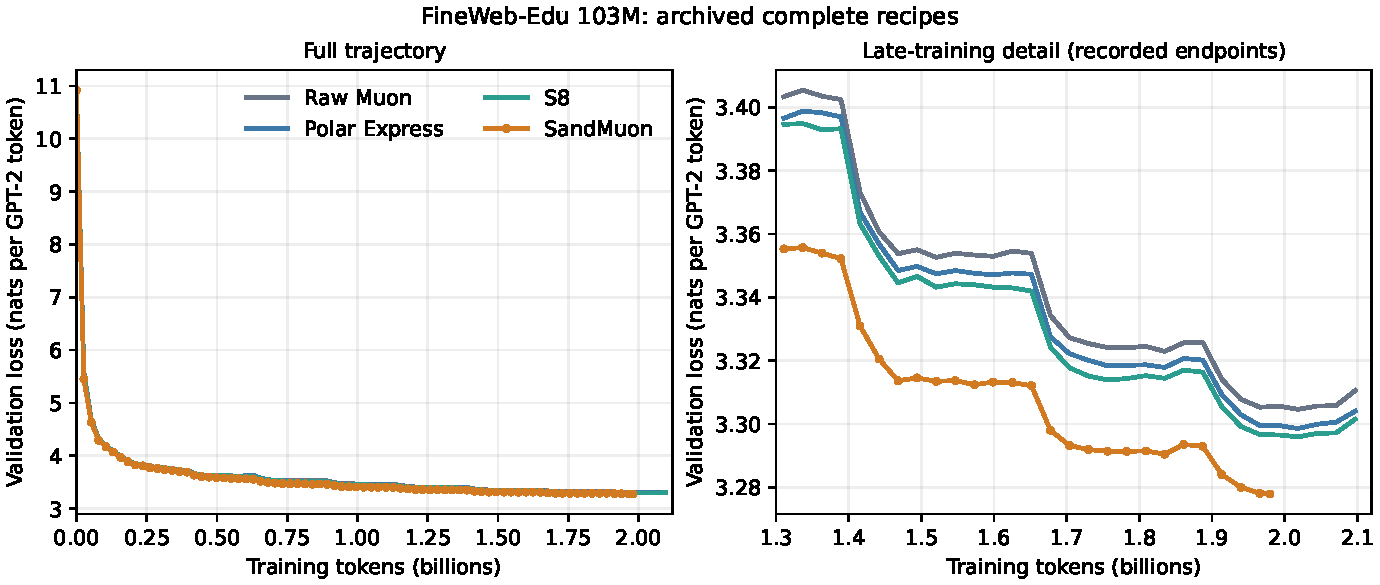
\includegraphics[width=0.97\linewidth]{figures/loss_vs_tokens.pdf}
\caption{Validation loss against consumed GPT-2 tokens for vanilla Muon, Polar Express, S8, and rank-one SAND-Muon. The three archived references end at 2.097B tokens, while SAND ends at 1.980B; their recorded training durations differ. The figure is descriptive evidence across four distinct single-run recipes.}
\label{fig:training}\end{figure}

\subsection{Centered-FP32 geometry screen}
A separate Kaggle pilot on a Tesla T4 compared ten centered-FP32 arms for 1,000 updates at seed 1337. Each arm used a four-layer, width-320 model with approximately 21,055,680 total parameters, including 4,915,200 SAND matrix parameters and 16,140,480 auxiliary AdamW parameters. It used context 128 and the same pinned FineWeb-Edu GPT-2-token revision as the production run. The reported endpoint losses for the reference, diagonal activation weighting, aligned geometry, and tempered output weighting were 5.871900, 5.864832, 5.883294, and 5.867986, respectively. Both the pilot and production run accumulated full-batch statistics; they differ in precision and in model, batch, context, and training horizon. These values screen implementation choices; they do not estimate a production effect or validate the BF16 production recipe.

\begin{figure}[!htbp]\centering
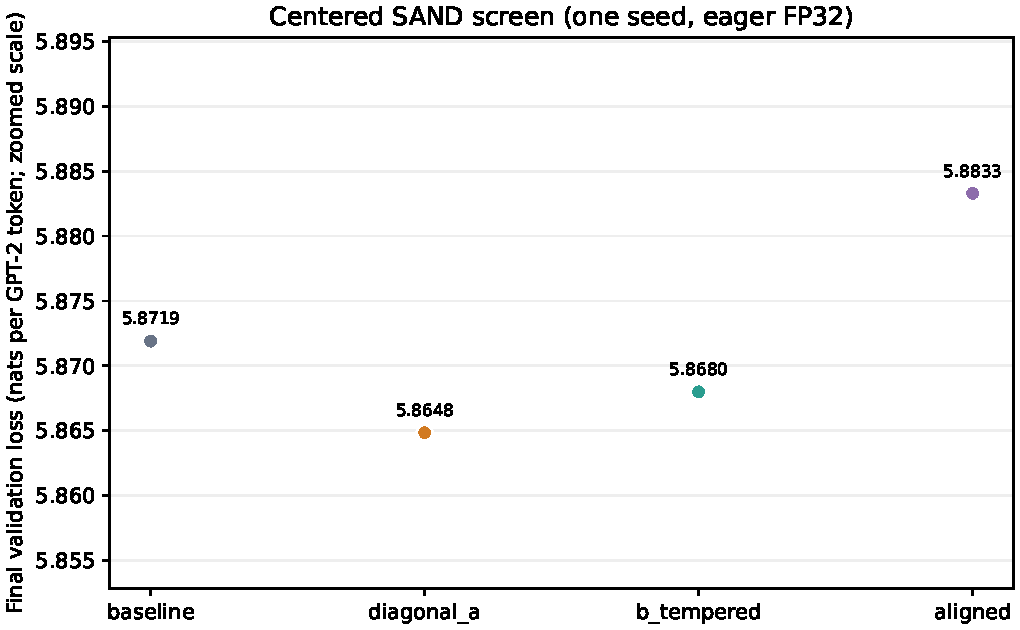
\includegraphics[width=0.93\linewidth]{figures/centered_screen_ablation.pdf}
\caption{Centered-FP32 1,000-update pilot outcomes for the baseline, diagonal-A, B-tempered, and aligned arms. These screening runs are not production-equivalent comparisons and are shown separately from the FineWeb-Edu main run.}
\label{fig:pilot}\end{figure}

\section{Discussion}
The case study demonstrates that a low-memory layerwise geometry can be integrated with a finite-stage spectral optimizer at 103M scale. At nearly equal recorded training durations, its endpoint validation loss is 0.026125 nats below the archived PE reference. The rank-one representation makes one non-diagonal activation correction cheap to apply. These are implementation and single-run observations. They do not show that activation means, output sensitivities, S8, or any one recipe choice caused the endpoint gap.

There are several limits to interpretation. First, the single-seed comparison has no estimate of run-to-run variation. Second, the endpoint uses different token counts and independently recorded runs; measured train time excludes evaluation and checkpoint activity and does not establish a same-device speed advantage. Third, SAND changes momentum, matrix transform, auxiliary AdamW settings, and the schedule alongside the geometry. Fourth, a centered-FP32 screen is not a BF16 production validation. Fifth, the cotangent statistic is observed-label squared sensitivity, not a Fisher estimate, and diagonal-plus-rank-one input geometry omits general activation covariance structure. Finally, the exact weighted-oracle argument applies to fixed factors and an exact polar map; the implementation uses moving estimates, momentum, finite polynomial arithmetic, and grafting.

The next evidence should isolate the geometry with paired seeds and identical optimizer details, compare the rank-one factor to diagonal-only and identity controls, include MALT and other diagonal preconditioners under one code path, and measure factor collection, update, and full-step costs on the same device. A separate evaluation stream and checks across model sizes would help determine whether the endpoint observation persists beyond this one training trajectory.

\section{Conclusion}
\SAND combines per-layer activation and observed-loss sensitivity statistics with a compensated finite polar update. Its diagonal-plus-rank-one activation model admits analytic inverse-square-root actions, while the idealized whitened polar map has a direct weighted spectral-oracle interpretation. One 103M FineWeb-Edu run completed under an approximately 37,809-second update-time budget and ended at validation loss 3.277938. The archived PE run ended at 3.304063 after nearly the same recorded update time but more tokens and a different complete recipe. This result supports further controlled evaluation of the geometry; it is not evidence of general optimizer superiority or an isolated causal gain.

\paragraph{Artifacts.} The standalone implementation, historical GPU-source archive, manuscript, validation traces, and reproducibility records are available at \url{https://github.com/pxike/SandMuon}. The package distinguishes the tested GPU implementation from its portable FP32 reference. The S8 component is also documented at \url{https://github.com/pxike/S8Muon}. A source bundle accompanies this draft as \texttt{SandMuon\_source.zip}.

\section*{Acknowledgements}
The author used language-model assistance for drafting and software development, and takes full responsibility for the methodology, experiments, and manuscript.

\bibliographystyle{plainnat}
\bibliography{references}

\appendix
\section{Reproduction and implementation details}\label{app:repro}
The production output is \path{vast_outputs/20260922-105255-736706896/benchmarks/sand_rank1_fineweb_timebudget}. Its manifest records the model configuration, dataset revision, seed, batch, optimizer, precision, GPU, software version, source hashes, and validation reference. The budget record reports 15,106 updates, 1,979,973,632 tokens, 37,808.941665 s of measured training time, and a 1.269320 s overshoot of the target budget. The current \path{odl/optim/diagonal_weighted_pe.py} and packed-prefix S8 source hashes agree with the manifest. The runner hash in the old manifest differs from the current runner, so the preserved manifest and traces are the primary run record rather than a claim of exact end-to-end reconstruction. The measured clock includes synchronized updates and data transfer; it excludes validation, checkpoint I/O, startup, and discarded compilation warmup.

For a matrix parameter with stored dimensions $o\times d$, the production optimizer accumulates activation and cotangent statistics through forward and backward hooks. The query projection's activation state is reused for the key and value projections in each attention block. The EMA coefficient is fixed at $0.97$ and state is updated once per optimizer step after all microbatches have contributed. The activation and cotangent state requires $O(d+o)$ persistent values per matrix, beyond momentum and polarization state. Collecting the statistics costs $O(N(d+o))$ over $N$ activation rows, while diagonal and rank-one factor actions on a dense matrix cost $O(od)$. Polarization additionally requires dense matrix products; these operation counts do not establish end-to-end overhead. The nonsymmetric whitening actions use diagonal scaling and vector inner products, so no dense covariance factor is stored. Matrix momentum and Nesterov source use coefficients $0.8$. The whitened matrix batches are polarized with five S8 stages. The first stage uses compensated BF16 matrix products with FP32 accumulation and temporaries, and the output is mapped back with the transpose-paired whitening factors before Frobenius grafting to $\sqrt{o}$.

The SAND run and PE reference use the same pinned FineWeb-Edu GPT-2-token revision, 103,176,192-parameter model configuration, seed value 1337, effective batch 128, microbatch 16, context 1,024, peak matrix LR 0.01, RTX 3090 model, and validation protocol according to their manifests. Their schedules differ by design: PE decays over 16,000 updates, while SAND decays over the reference training-time budget and stops at that budget. The historical S8 and vanilla-Muon rows in Table~\ref{tab:endpoints} come from the separate three-arm S8 paper and are context only.

\subsection{Finite polar recipe and released code}
In exact arithmetic, the five-stage S8 map first orients a matrix $Z$ so its smaller dimension indexes the Gram matrix and initializes
\begin{equation}
 X_0=Z/(1.35\|Z\|_{S_8}),\qquad
 \|Z\|_{S_8}=\|(ZZ^\top)^2\|_F^{1/4}.
\end{equation}
Its stages are $X_{j+1}=(a_j I+b_jX_jX_j^\top+c_j(X_jX_j^\top)^2)X_j$. The deployed coefficients are shown in Table~\ref{tab:coefficients}; the full-precision values and original coefficient manifest accompany the code. Production initially rounds the input through BF16, uses compensated products with FP32 accumulation and temporaries for the first stage, and ordinary BF16 products in subsequent stages. These arithmetic choices make the recorded implementation different from an eager FP32 evaluation of the same polynomial.
\begin{table}[ht]\centering
\caption{The S8 coefficient schedule used in the 103M SAND run (rounded for display). No additional output multiplier is used.}
\label{tab:coefficients}
\begin{tabular}{rrrr}\toprule
Stage & $a_j$ & $b_j$ & $c_j$\\\midrule
1 & 11.06212628 & $-56.05165323$ & 72.32081108\\
2 & 4.10072007 & $-2.93241832$ & 0.53396921\\
3 & 3.93031019 & $-2.87350979$ & 0.53665575\\
4 & 3.28056797 & $-2.41492559$ & 0.48635135\\
5 & 2.28274158 & $-1.63022966$ & 0.40275721\\\bottomrule
\end{tabular}\end{table}

The standalone package supplies an eager FP32 reference and preserves the historical GPU optimizer and kernel dependency closure separately. The reference generalizes layer selection to ordinary PyTorch linear modules, retains the historical GPT selection as an explicit option, and guards all-zero diagonal statistics with a positive normalized floor. These are documented release adaptations, not retrospective changes to the reported GPU experiment. CPU tests check dense whitening and transpose map-back, effective-batch accumulation, save/resume, zero signals, and the $\sqrt{o}$ update norm for square, tall, and wide matrices. No GPU throughput or training result is attributed to the new reference implementation.

\section{Application feasibility runs}
Two aesthetic-generation jobs provide additional single-optimizer feasibility examples. The pixel generator resumed from a saved checkpoint; the transformer generator started from random initialization. Both used the S8 polynomial with FP16 CUDA GEMMs on a Turing/T4 fallback path. They differ from the BF16 FineWeb production recipe and include no optimizer controls, so they do not support a comparative optimizer claim.
\begin{table}[h]
\centering
\caption{Single-optimizer application demonstrations. Runs differ in architecture and initialization; these reward values are not an optimizer comparison.}
\label{tab:applications}
\resizebox{\linewidth}{!}{%
\begin{tabular}{lrrrrl}
\toprule
Task & Parameters & Updates & Runtime (s) & Best adjusted reward & Final adjusted reward\\
\midrule
Pixel generator & 12,768,259 & 10,000 & 16,768 & 1.8601 & 1.1855\\
Transformer generator & 12,570,048 & 10,000 & 30,899.9 & 2.7186 & 2.5312\\
\bottomrule
\end{tabular}}
\end{table}

\section{Prioritized follow-up matrix}
Table~\ref{tab:next} lists the minimum controls needed to sharpen the central empirical claim.
\begin{table}[h]
\centering
\caption{Follow-up evidence needed to isolate the geometry and implementation cost.}
\label{tab:next}
\begin{tabular}{p{0.24\linewidth}p{0.69\linewidth}}
\toprule
Question & Control or measurement\\
\midrule
Does the endpoint gap reproduce? & At least three paired seeds with identical model initialization protocol, token budget, schedule, software stack, and validation stream.\\
Which statistic matters? & Identity, diagonal activation, rank-one activation, diagonal cotangent, and combined geometry under the same S8, momentum, graft, and auxiliary optimizer.\\
How does SAND compare with related geometry? & MALT-style diagonal controls and an exact implementation of the published recipes, with matched training details and no retrospective hyperparameter changes.\\
What is the cost? & Same-device measurements of statistic collection, factor refresh, polarization, map-back, and complete optimizer-step time, with evaluation and startup accounted for separately.\\
Does the result travel? & An independent validation stream and at least one additional model size or architecture.\\
\bottomrule
\end{tabular}
\end{table}

\end{document}
